% ===================== 7. PARAMETER TUNING =====================
\section{Phân tích độ nhạy và tinh chỉnh tham số (Parameter Tuning)}
\label{sec:tuning}

Mỗi tham số của ALNS được biện minh bằng đồ thị độ nhạy, không phải chọn tùy ý.
Mọi thí nghiệm chạy trên instance nghẽn \texttt{test09} ($N{=}200$, $M{=}5$) ---
nơi động lực học bộc lộ rõ nhất --- lấy trung bình $5$ hạt giống ngẫu nhiên.

\subsection{Sự tiến hóa của xác suất chọn toán tử (cân bằng Khám phá -- Khai thác)}
\begin{figure}[H]
  \centering
  \begin{subfigure}{0.49\textwidth}
    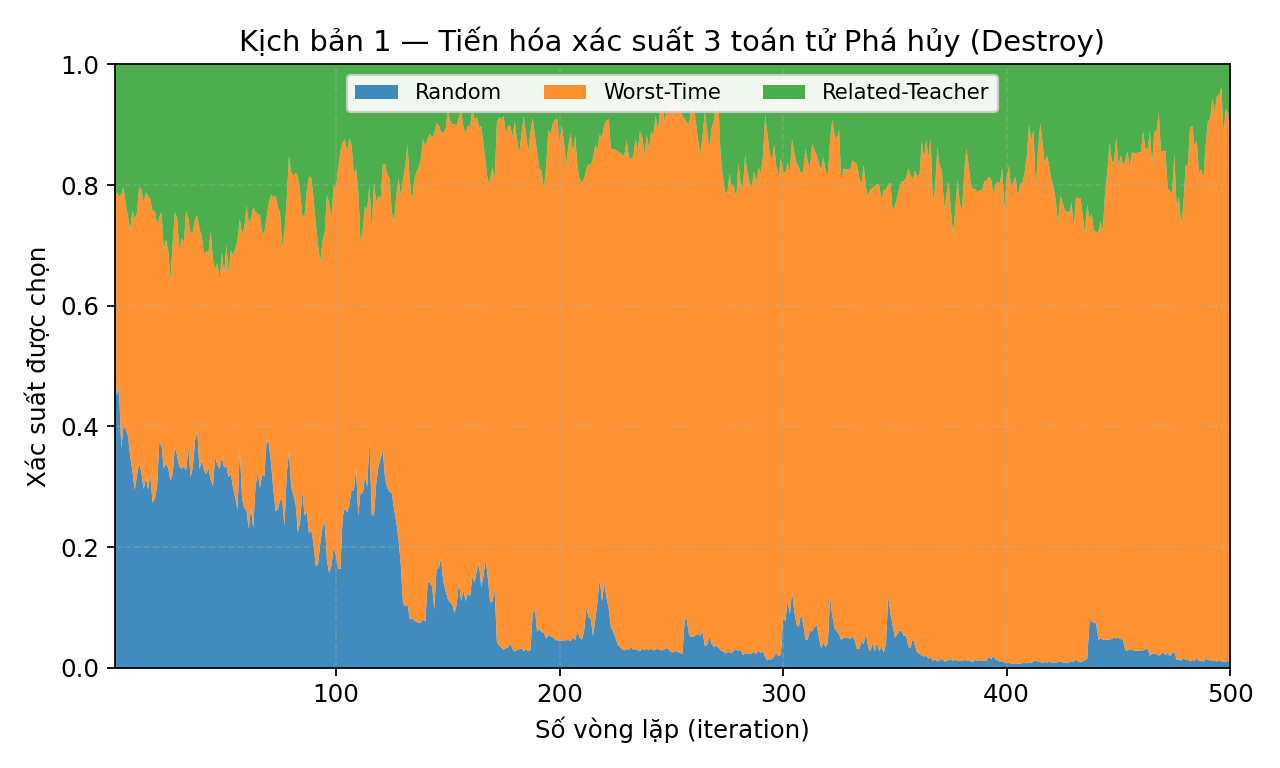
\includegraphics[width=\linewidth]{figures/s1_destroy_probability.png}
    \caption{Toán tử Phá hủy}
  \end{subfigure}\hfill
  \begin{subfigure}{0.49\textwidth}
    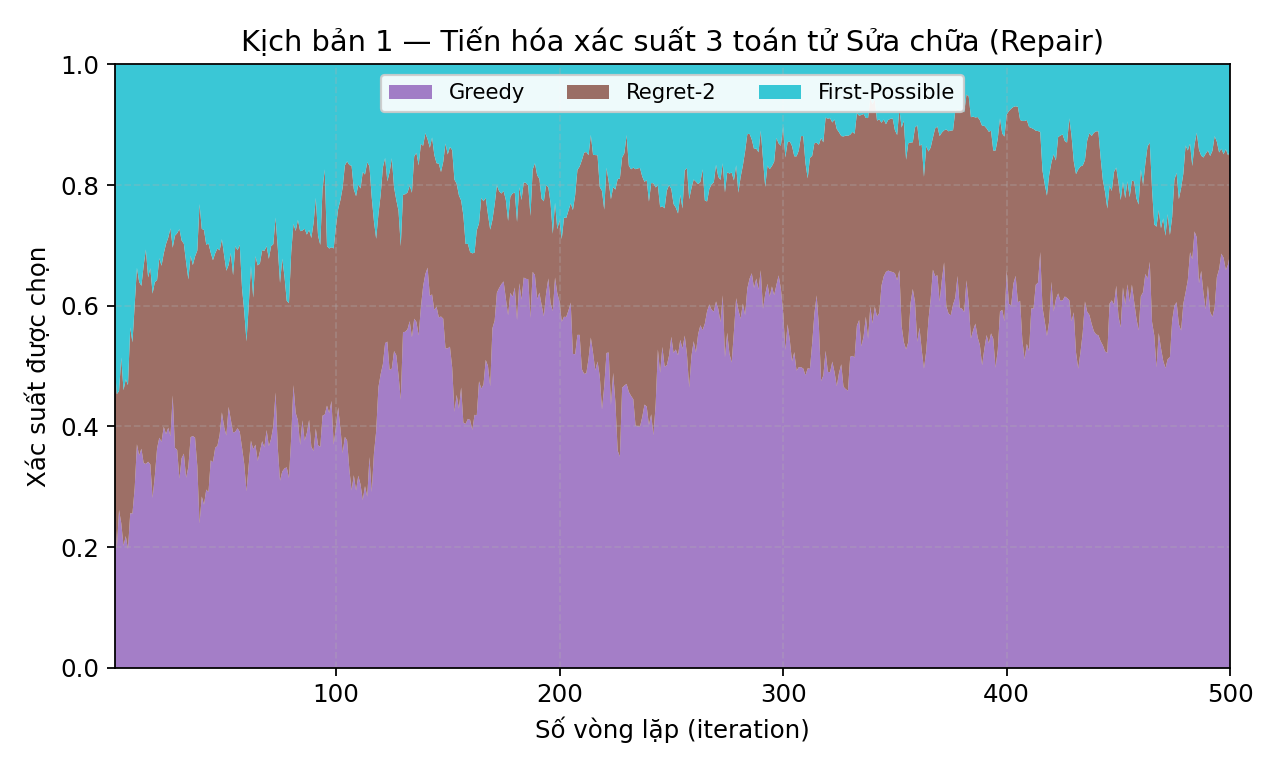
\includegraphics[width=\linewidth]{figures/s1_repair_probability.png}
    \caption{Toán tử Sửa chữa}
  \end{subfigure}
  \caption{Miền xác suất chọn toán tử theo vòng lặp (tổng mỗi cột $=1$), tính
  theo~\eqref{eq:roulette}.}
  \label{fig:s1}
\end{figure}

\noindent Hình~\ref{fig:s1} cho thấy cơ chế thích nghi \emph{thực sự học}: khởi đầu
gần đồng đều (giai đoạn \emph{khám phá}), thuật toán nhanh chóng dồn xác suất cho
\opt{Worst-Time} (tỉ trọng cuối $\approx 0.89$) và \opt{Greedy} bên sửa chữa
($\approx 0.69$) --- giai đoạn \emph{khai thác} chiến lược hiệu quả nhất trên
instance nghẽn phòng, trong khi phá ngẫu nhiên bị đào thải. Đây là minh chứng định
lượng cho giá trị của adaptive selection.

\subsection{Tác động của hệ số học $\lambda$ (Learning Rate)}
\begin{figure}[H]
  \centering
  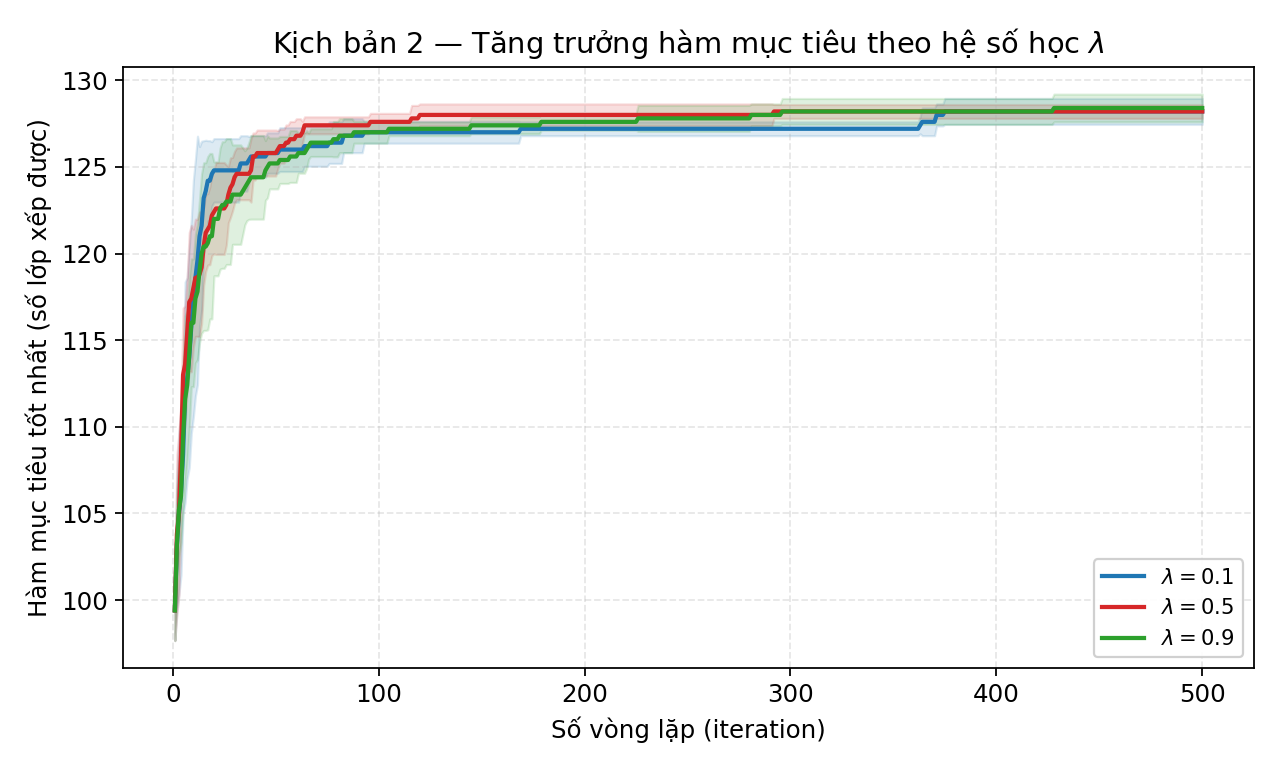
\includegraphics[width=0.70\textwidth]{figures/s2_lambda_convergence.png}
  \caption{Tăng trưởng hàm mục tiêu theo $\lambda\in\{0.1,0.5,0.9\}$; dải mờ là
  $\pm 1$ độ lệch chuẩn trên $5$ hạt giống.}
  \label{fig:s2}
\end{figure}

\noindent Ba giá trị cho chất lượng trung bình gần như nhau ($\approx 128$ lớp),
nên tiêu chí phân định là \emph{độ ổn định}: $\lambda{=}0.5$ cho độ lệch chuẩn cuối
kỳ ($\sigma\approx 0.40$) nhỏ hơn $\sim 2\times$ so với $\lambda{=}0.1$ (quên nhanh,
$\sigma\approx 0.75$) và $\lambda{=}0.9$ (ì, $\sigma\approx 0.80$). Ta chọn
$\boxed{\lambda=0.5}$ vì hành vi tái lập và đáng tin cậy nhất.

\subsection{Sự biến thiên Nhiệt độ $T$ và hệ số làm mát $\alpha$ (Cooling Schedule)}
\begin{figure}[H]
  \centering
  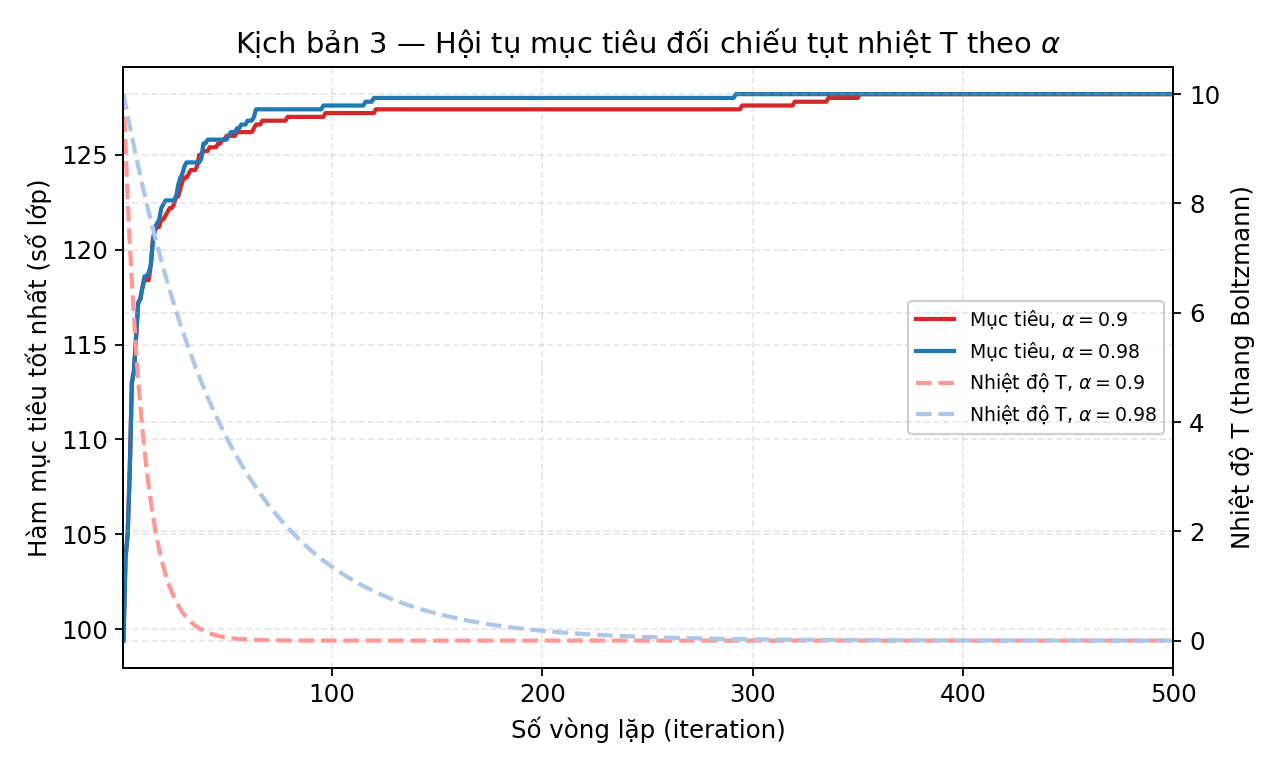
\includegraphics[width=0.76\textwidth]{figures/s3_temperature_dualaxis.png}
  \caption{Đồ thị kép: hội tụ mục tiêu (đường liền, trục trái) đối chiếu tụt nhiệt
  $T$ (đường đứt, trục phải) cho $\alpha=0.90$ và $\alpha=0.98$.}
  \label{fig:s3}
\end{figure}

\noindent Với $\alpha{=}0.90$, nhiệt độ rơi về $\approx 0.06$ chỉ sau $\sim 50$
vòng --- sau đó $e^{-\Delta/T}\approx 0$, thuật toán \emph{đóng băng} thành leo đồi
thuần túy, dễ chết yểu ở cực trị cục bộ. Với $\alpha{=}0.98$, $T$ còn $\approx 3.7$
tại vòng $50$ và chỉ tiệm cận $0$ quanh vòng $250$, giữ ``van xả'' khám phá lâu hơn
mà gần như không tốn thêm chi phí. Ta chọn $\boxed{T_0=10,\ \alpha=0.98}$.
